\pagebreak
\subsection{Adaptive Iterations}
[15\%] Perform adaptive iterations for $\alpha = [0.5, 1, 1.5, 2, 2.5, 3]$ degrees. Run the same number of adaptive iterations for each $\alpha$ at least 5. Plot the ATPR output from your finest mesh versus alpha, and discuss the trend. Include flowfield plots to augment your discussion.

\subsubsection{ATPR Versus Angle of Attack}
\begin{figure}[h]
    \centering
    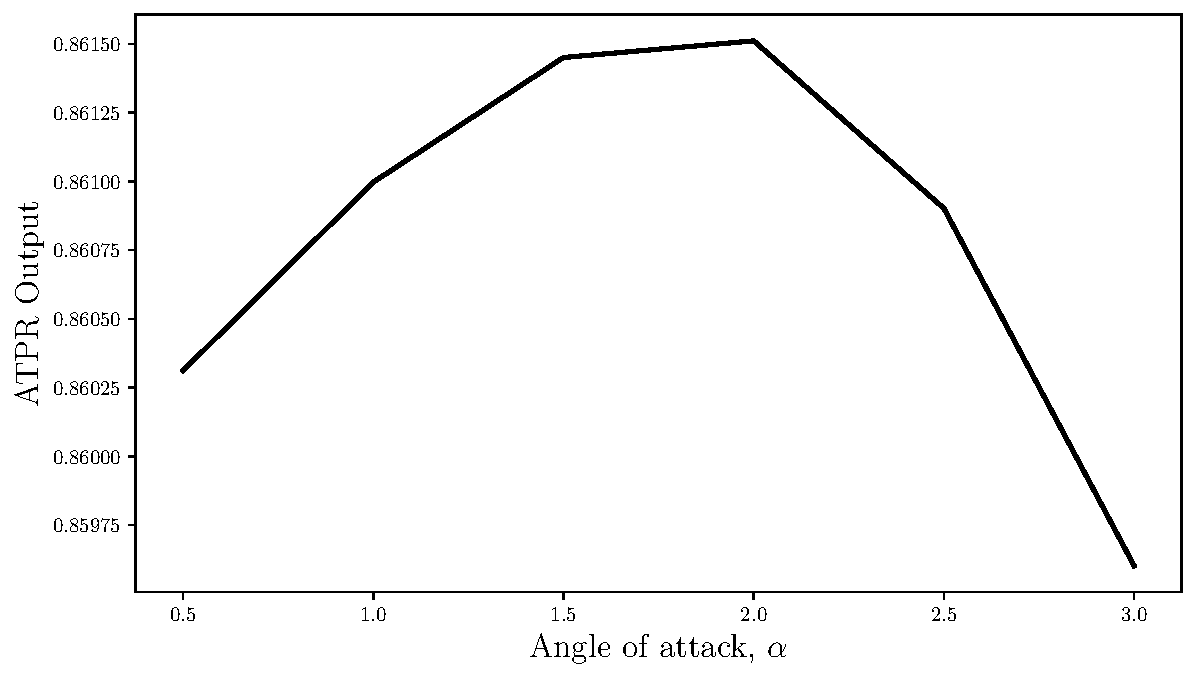
\includegraphics[width = 0.9\linewidth]{rep/q5/ATPR.pdf}
    \caption[ATPR and Angle of Attack]{Effects of varying $\alpha$ on the ATPR output.}
    \label{fig:aoa_ATPR}
\end{figure}
\textcolor{red}{\large PLACE HOLDER}

\pagebreak
\subsubsection{Flow Fields for Varyin Angle of Attacks}

\begin{figure}[h]
    \centering
    \begin{subfigure}[h]{0.32\linewidth}
        \centering
        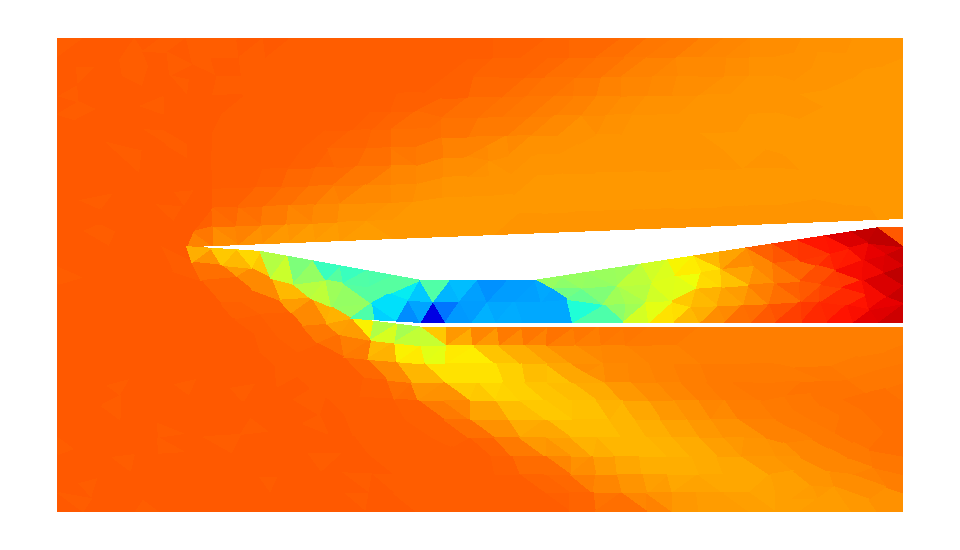
\includegraphics[width=\linewidth]{rep/q5/mach_a5.pdf}
        \caption{Mach field at $\alpha=0.5\degree$.}
    \end{subfigure}
    \begin{subfigure}[h]{0.32\linewidth}
        \centering
        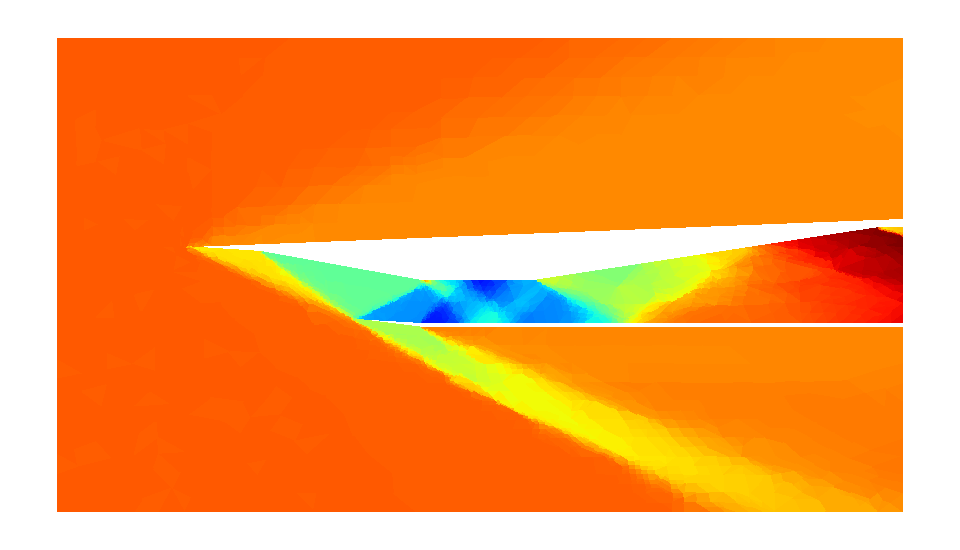
\includegraphics[width=\linewidth]{rep/q5/mach_a10.pdf}
        \caption{Mach field at $\alpha=1.0\degree$.}
    \end{subfigure}
    \begin{subfigure}[h]{0.32\linewidth}
        \centering
        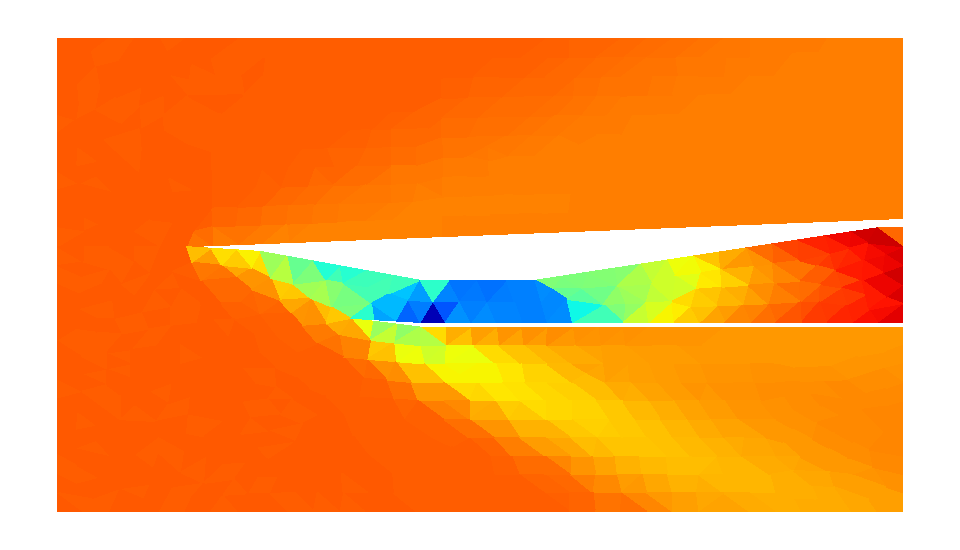
\includegraphics[width=\linewidth]{rep/q5/mach_a15.pdf}
        \caption{Mach field at $\alpha=1.5\degree$.}
    \end{subfigure}

    \begin{subfigure}[h]{0.32\linewidth}
        \centering
        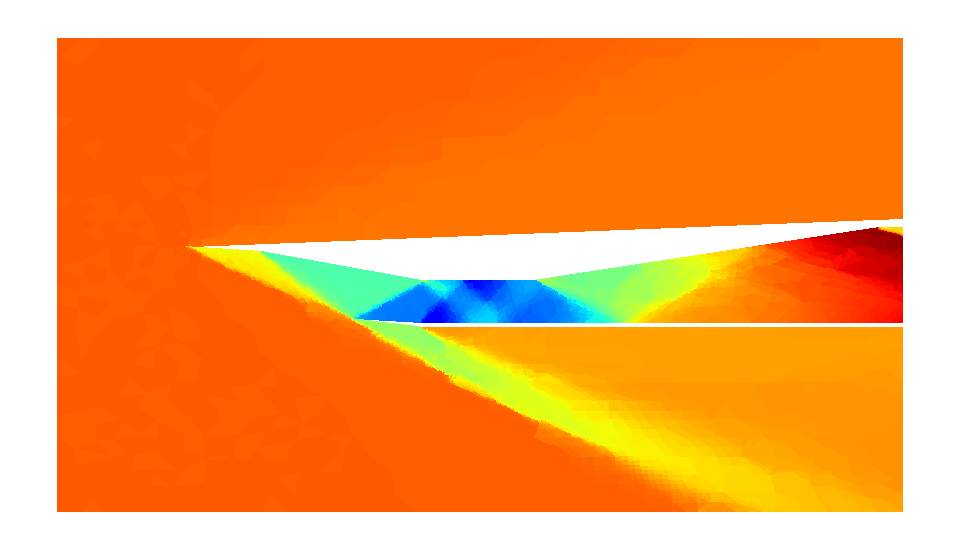
\includegraphics[width=\linewidth]{rep/q5/mach_a20.pdf}
        \caption{Mach field at $\alpha=2.0\degree$.}
    \end{subfigure}
    \begin{subfigure}[h]{0.32\linewidth}
        \centering
        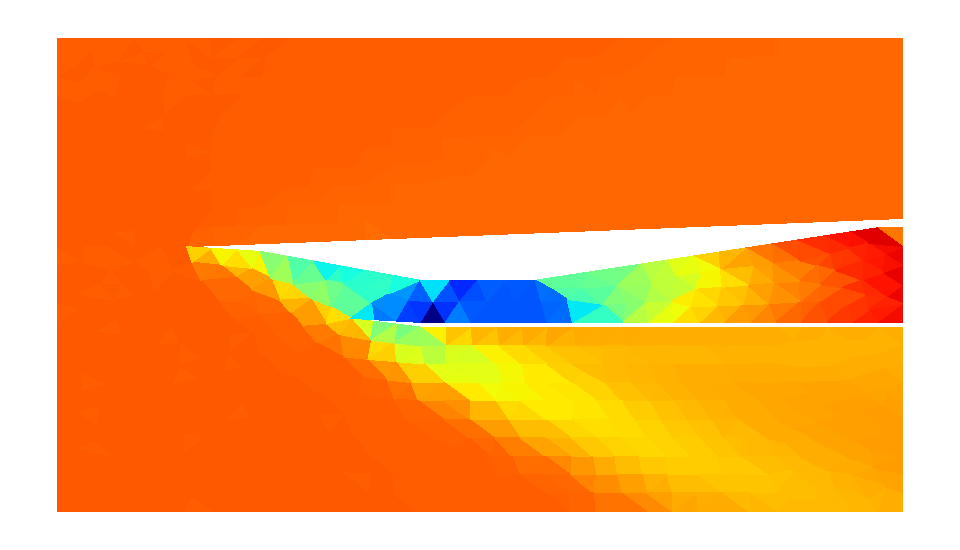
\includegraphics[width=\linewidth]{rep/q5/mach_a25.pdf}
        \caption{Mach field at $\alpha=2.5\degree$.}
    \end{subfigure}
    \begin{subfigure}[h]{0.32\linewidth}
        \centering
        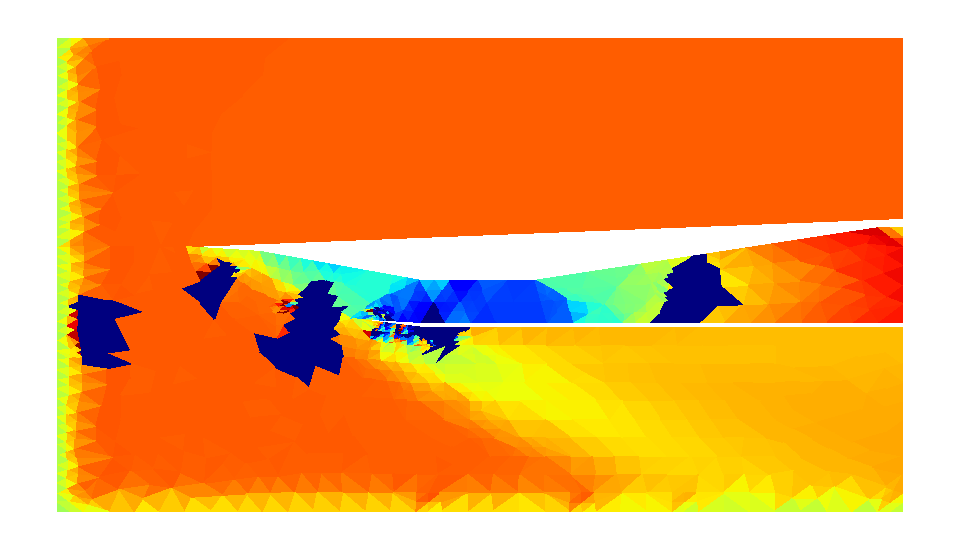
\includegraphics[width=\linewidth]{rep/q5/mach_a30.pdf}
        \caption{Mach field at $\alpha=3.0\degree$.}
    \end{subfigure}
    \caption[Mach Field with Varying Angle of Attack]{Varying angle of attack, and its effect on the mach field.}
\end{figure}

\paragraph{Effect on Mach Field from Varying Angle of Attack}
\textcolor{red}{\large PLACE HOLDER}

\pagebreak
\begin{figure}[h]
    \centering
    \begin{subfigure}[h]{0.32\linewidth}
        \centering
        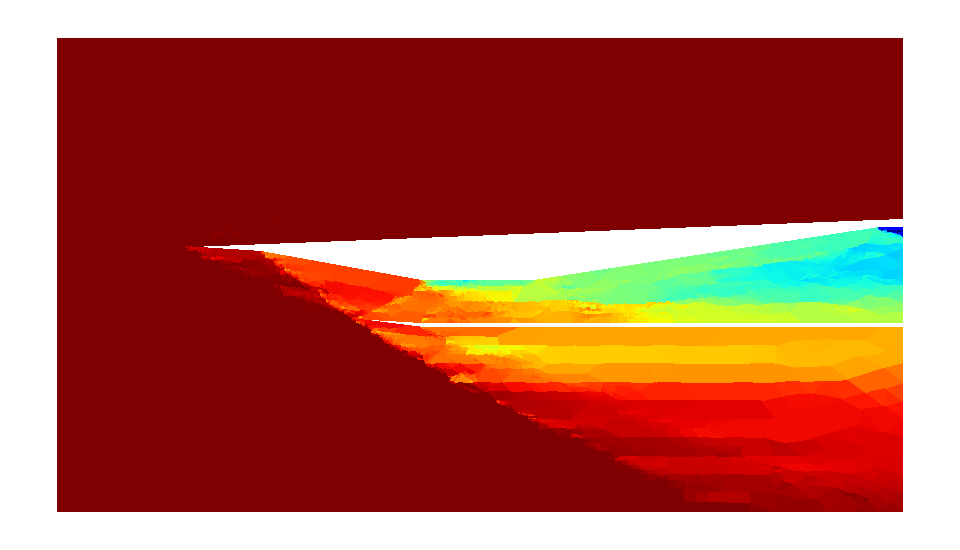
\includegraphics[width=\linewidth]{rep/q5/pt_a5.pdf}
        \caption{Total pressure field at $\alpha=0.5\degree$.}
    \end{subfigure}
    \begin{subfigure}[h]{0.32\linewidth}
        \centering
        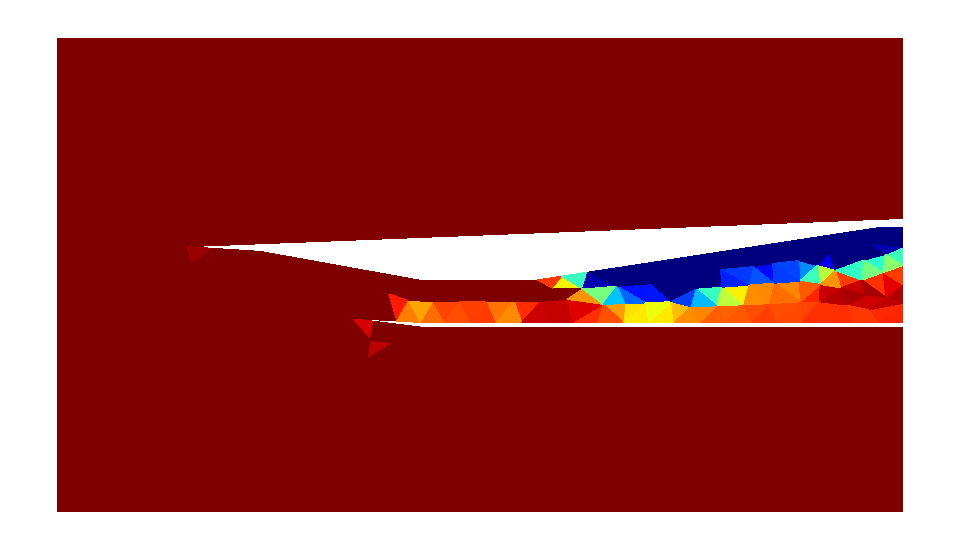
\includegraphics[width=\linewidth]{rep/q5/pt_a10.pdf}
        \caption{Total pressure field at $\alpha=1.0\degree$.}
    \end{subfigure}
    \begin{subfigure}[h]{0.32\linewidth}
        \centering
        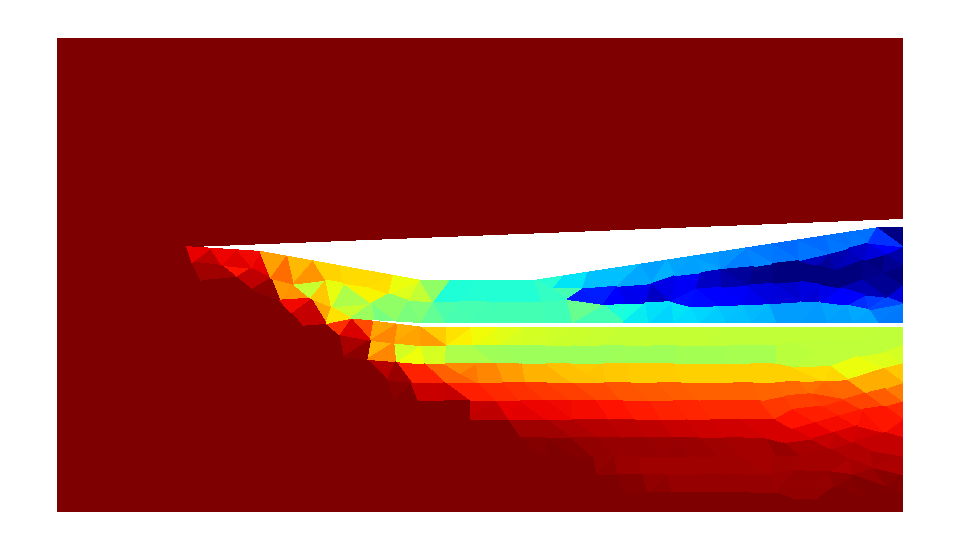
\includegraphics[width=\linewidth]{rep/q5/pt_a15.pdf}
        \caption{Total pressure field at $\alpha=1.5\degree$.}
    \end{subfigure}

    \begin{subfigure}[h]{0.32\linewidth}
        \centering
        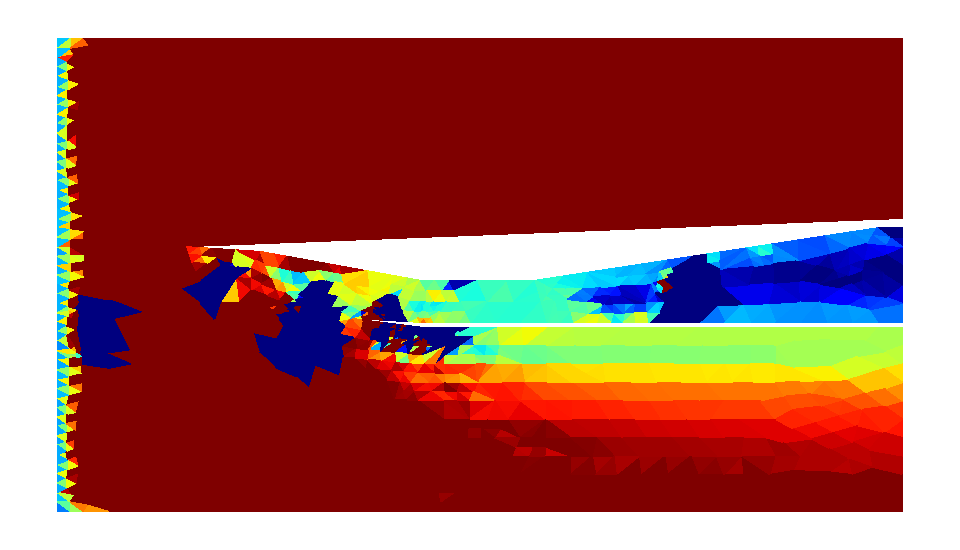
\includegraphics[width=\linewidth]{rep/q5/pt_a20.pdf}
        \caption{Total pressure field at $\alpha=2.0\degree$.}
    \end{subfigure}
    \begin{subfigure}[h]{0.32\linewidth}
        \centering
        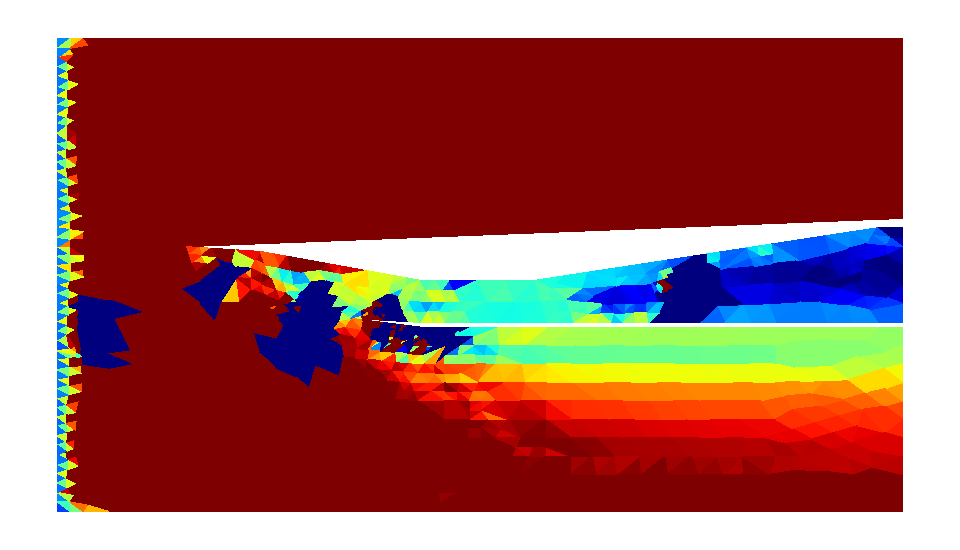
\includegraphics[width=\linewidth]{rep/q5/pt_a25.pdf}
        \caption{Total pressure field at $\alpha=2.5\degree$.}
    \end{subfigure}
    \begin{subfigure}[h]{0.32\linewidth}
        \centering
        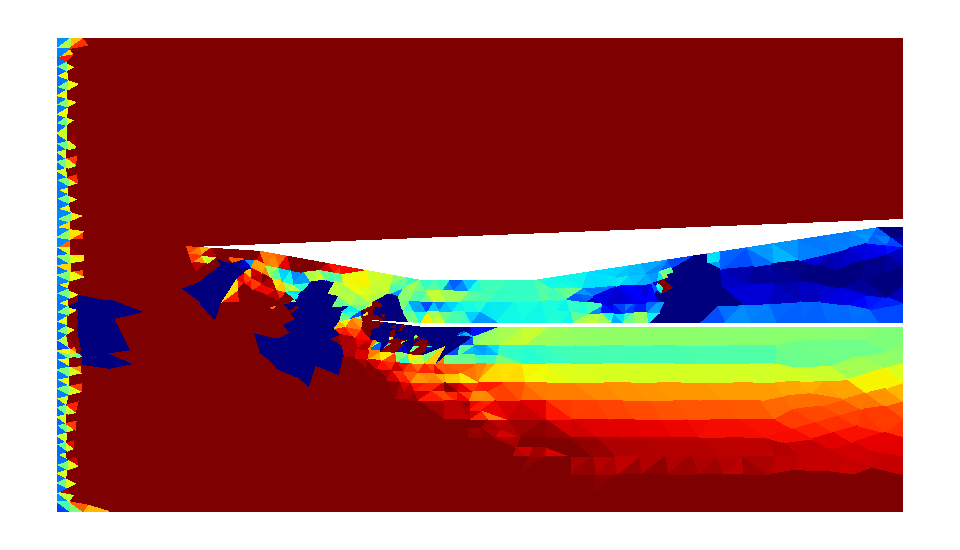
\includegraphics[width=\linewidth]{rep/q5/pt_a30.pdf}
        \caption{Total pressure field at $\alpha=3.0\degree$.}
    \end{subfigure}
    \caption[Total Pressure Field with Varying Angle of Attack]{Varying angle of attack, and its effect on the total pressure field.}
\end{figure}

\paragraph{Effect on Total Pressure Field from Varying Angle of Attack}
\textcolor{red}{\large PLACE HOLDER}